\documentclass[aps,prb,twocolumn,superscriptaddress,amsmath,amssymb]{revtex4-2}
\usepackage{graphicx}
\usepackage{bm}
\usepackage{xcolor}
\newcommand{\Nmu}{N_\mu}
\newcommand{\cmu}{c_\mu}
\newcommand{\rr}{\mathbf{r}}
\newcommand{\GG}{\mathbf{G}}
\newcommand{\kk}{\mathbf{k}}
\newcommand{\qq}{\mathbf{q}}
\newcommand{\todo}[1]{\textcolor{red}{[TODO: #1]}}

\begin{document}

\title{Coulomb-metric point selection in interpolative separable density fitting}

\author{Miguel A. Morales}
\affiliation{Center for Computational Quantum Physics, Flatiron Institute, New York, NY 10010, USA}

\date{\today}

\begin{abstract}
Interpolative separable density fitting (ISDF) factorizes the two-electron
Coulomb tensor at a cost that scales with the number of interpolation points
$\Nmu = \cmu N_{\rm orb}$, with every downstream object in the auxiliary index
costing $O(\Nmu^2)$ in storage and $O(\Nmu^3)$ in dense linear algebra.
Standard ISDF selects interpolation points by a pivoted Cholesky factorization
of the orbital-pair overlap metric, which optimally resolves pair densities in
the $L^2$ sense but over-resolves short-wavelength structure that the Coulomb
kernel suppresses. We show that, because the grid metric cancels exactly from
the ISDF least-squares solve, the metric can influence the factorization
\emph{only} through the choice of interpolation points and through pair-space
weights, and we introduce three composable, input-driven modifications of the
selection: (i) separable pair-space weighting of the selection Gram matrix,
(ii) a Gaussian-filtered orbital surrogate, and (iii) an exact two-pass
Coulomb-metric re-ranking of an inflated candidate pool. None of them alter
the ISDF ansatz, the interpolation-vector solve, or any downstream consumer,
and each reduces to the standard algorithm in a well-defined limit. On silicon
we measure the error in the Hartree, exact-exchange, and RPA correlation
energies as a function of $\cmu$ and find \todo{summary of findings: reduction
of $\cmu^*$ at fixed accuracy, per knob and composed}. The re-ranking pass
adds only a factor $s\sim 2$ to the selection cost, which is itself a small
fraction of the total calculation.
\end{abstract}

\maketitle

\section{Introduction}
\label{sec:intro}

The interpolative separable density fitting (ISDF), or tensor hypercontraction
(THC), representation of the two-electron repulsion integrals underlies
low-scaling implementations of Hartree--Fock exchange, MP2 and RPA correlation
energies, coupled-cluster methods, $GW$ and related many-body perturbation
frameworks, and quantum-algorithm resource estimates
\todo{cite: Lu-Ying 2015, Hu-Lin-Yang 2017, Parrish-Hohenstein-Martinez THC,
Malone-Lee QC resource, CoQui}.  In all of these, the auxiliary
(interpolation-point) index carries the factorization,
\begin{equation}
  \rho_p(\rr) \equiv u^*_i(\rr) u_a(\rr)
  \;\approx\; \sum_{\mu=1}^{\Nmu} \zeta_\mu(\rr)\, \rho_p(\rr_\mu),
  \label{eq:isdf}
\end{equation}
so that any object stored on the auxiliary index costs $O(\Nmu^2)$ and any
factorization or inversion there costs $O(\Nmu^3)$.  The proportionality
constant $\cmu = \Nmu/N_{\rm orb}$ at fixed target accuracy is therefore the
single most important number in the method: reducing $\cmu$ from 10 to 6 is a
factor $2.8$ in auxiliary storage and $4.6$ in dense linear algebra,
everywhere at once.

Standard ISDF chooses the points $\{\rr_\mu\}$ by pivoted Cholesky
factorization of the pair-density overlap (Gram) matrix, which minimizes the
$L^2$ error of the fitted pair densities greedily. That objective treats all
Fourier components of the pair density equally, while every consumer of the
factorization contracts it against the Coulomb kernel
$v(\GG) = 4\pi/|\GG|^2$ (or a screened variant), which discounts
short-wavelength errors by two powers of $|\GG|$.  The overlap-selected point
set consequently spends resolution where the target quantity does not need it.
\todo{1-2 sentences on prior work on weighted/centroid selection: centroidal
Voronoi ISDF, machine-learned selection, if citing.}

In this paper we adapt the point selection --- and only the point selection ---
to the Coulomb metric.  The starting observation
(Sec.~\ref{sec:cancellation}) is that the ISDF interpolation vectors are
independent of any grid-space metric: the metric cancels identically from the
least-squares solve.  All freedom therefore resides in (a) \emph{which} points
are selected and (b) pair-space weights.  We exploit this with three
independent, composable knobs (Sec.~\ref{sec:knobs}), all reusing the
existing pivoted-Cholesky machinery, all controlled from the input file, and
all reducing bitwise to the standard algorithm in their default settings.
Section~\ref{sec:results} measures the resulting error in the Hartree,
exact-exchange, and RPA correlation energies of silicon as a function of
$\cmu$, for norm-conserving, ultrasoft, and PAW pseudopotentials.

\section{Theory}
\label{sec:theory}

\subsection{ISDF and the exact cancellation of the grid metric}
\label{sec:cancellation}

Collect the pair densities on the real-space grid in
$Z \in \mathbb{C}^{N_g \times N_{\rm pair}}$, $Z_{gp} = \rho_p(\rr_g)$, and
let $\Theta = Z[I,:]$ be its restriction to the interpolation points
$I = \{\rr_\mu\}$. The ISDF ansatz \eqref{eq:isdf} is $Z \approx \zeta\,\Theta$
with $\zeta \in \mathbb{C}^{N_g\times \Nmu}$.  Minimizing the weighted
residual in an arbitrary (Hermitian, positive definite) grid metric $v$ and
pair weight $W = \mathrm{diag}(w_p)$,
\begin{equation}
  E \;=\; \mathrm{Tr}\!\left[ (Z-\zeta\Theta)\, W\, (Z-\zeta\Theta)^\dagger\, v \right],
\end{equation}
gives the stationarity condition
$v\,(Z-\zeta\Theta)\,W\,\Theta^\dagger = 0$, and since $v$ is invertible,
\begin{equation}
  \zeta \;=\; Z\,W\,\Theta^\dagger \left( \Theta\, W\, \Theta^\dagger \right)^{-1}.
  \label{eq:zeta}
\end{equation}
The grid metric $v$ \emph{cancels identically}; the pair weight $W$ does not.
The structural reason is that $\zeta$ carries a free grid index, so the
residual is driven orthogonal to the row space of $\Theta$ at every grid point
independently.  Three consequences shape everything that follows: the
$\zeta$ solve already in production is $v$-optimal for the given points; no
alternating or quartic-scaling optimization can improve it at fixed $I$; and
the metric can act only through the selection of $I$ and through $W$.

\subsection{The selection objective}
\label{sec:objective}

With $\zeta$ eliminated, the fit error in the metric $v$ as a function of the
point set is
\begin{equation}
  E_v(I) \;=\; \mathrm{Tr}\left[\, Q_\perp\, M \,\right],
  \qquad M = Z^\dagger v\, Z,
  \label{eq:objective}
\end{equation}
with $Q_\perp$ the projector onto the orthogonal complement of the selected
rows in pair space.  Greedy minimization of \eqref{eq:objective} is pivoted
Cholesky on
\begin{equation}
  K \;=\; Z\, M\, Z^\dagger \;=\; C\, v\, C, \qquad C = Z Z^\dagger,
  \label{eq:K}
\end{equation}
where $C_{gg'} = A_{gg'} \odot B^*_{gg'}$ has the Hadamard structure of a
product of orbital Gram matrices,
$A_{gg'} = \sum_i u_i(\rr_g)u_i^*(\rr_{g'})$, that makes its diagonal and
columns computable in $O(N_g N_{\rm orb})$.  Standard selection replaces
$M \to \mathbb{1}$, i.e.\ pivots on $C$ itself.  Pivoting on $K$ directly is
not affordable: $v$ is a convolution and does not commute with the Hadamard
structure, so a single column of $K$ costs $O(N_g N_i N_a)$ and the full
selection $O(N_g N_{\rm orb}^3)$.  The three knobs below approach the
$v$-weighted objective at essentially the cost of the standard one.

\subsection{Knob 1: separable pair-space weights}
\label{sec:knob1}

\todo{condense spec Sec. 2: separable weights preserve the Hadamard
structure at $N_L\times$ cost; PSD by the Schur product theorem for
$f_p, g_p, c_p \ge 0$; Laplace expansion for energy denominators;
selection-only by default; rotation-invariance caveat.}

\subsection{Knob 2: filtered-orbital surrogate}
\label{sec:knob2}

For point selection only, attenuate each orbital's plane-wave coefficients,
\begin{equation}
  \tilde c_{n\kk}(\GG) = c_{n\kk}(\GG)\,
  e^{-\alpha |\kk+\GG|^2 / G_c^2},
\end{equation}
with $G_c$ the wavefunction cutoff, build the selection Gram from the
$\tilde u$, pivot, then solve Eq.~\eqref{eq:zeta} with the \emph{unfiltered}
orbitals.  Filtering both factors of the pair density attenuates its
transform at roughly $\sqrt{2}$ smaller width with a Gaussian rather than
$1/G^2$ profile, so this is a surrogate for --- not an implementation of ---
the Coulomb metric; its virtue is that it costs one extra FFT sweep and
nothing else.  $\alpha=0$ recovers the standard algorithm exactly.

\subsection{Knob 3: exact Coulomb re-ranking of a candidate pool}
\label{sec:knob3}

Run the standard (or knob-1/2--modified) pivoted Cholesky to an inflated rank
$N_1 = \lceil s \Nmu \rceil$, $s\in[1.5,3]$, producing a candidate pool $P$
and the Cholesky factor $L \in \mathbb{C}^{N_g\times N_1}$.  Because the
Schur complement vanishes exactly on eliminated pivots,
$C[P,:] = L[P,:]\, L^\dagger \equiv \ell L^\dagger$ with
$\ell = L[P,:]$ lower triangular, one has, exactly,
\begin{equation}
  K_{PP} \;=\; \ell\, (L^\dagger v L)\, \ell^\dagger
        \;=\; Y^\dagger Y,
  \qquad Y = R\,\ell^\dagger,
  \label{eq:KPP}
\end{equation}
where $R(\GG,j) = \sqrt{\bar v(\GG)}\, \hat L(\GG,j)$ is assembled from the
Fourier transforms of the Cholesky columns and a pluggable multiplier
$\bar v(\GG)$ (bare, attenuated, $\qq$-averaged, or screened).  A dense
pivoted Cholesky of the $N_1\times N_1$ matrix $K_{PP}$ then re-ranks the
pool in the Coulomb metric and keeps the leading $\Nmu$ points.  The
$v$-optimum is searched only within the $L^2$-good pool --- re-ranking, not
re-searching --- which is what makes the cost a factor $\sim s$ on selection
with no change in scaling.  $s=1$ and $\bar v = 1$ are exact no-op limits.

\subsection{Implementation in CoQui}
\label{sec:implementation}

\todo{brief: pivoted-Cholesky driver anchors; options table (the nine
isdf\_* keys with defaults); bitwise-regression defaults; PAW consistency ---
augmentation channels already Coulomb-ranked, point selection now matches;
cost table from spec Sec. 4.4.}

\section{Results}
\label{sec:results}

\todo{Computational details: Si fcc, 2x2x2 (and 4x4x4 production) MP mesh,
NCPP/USPP/PAW, cutoffs, beta=1000 DLR, reference = Cholesky 1e-10 (NCPP) and
THC self-convergence (USPP/PAW). Error metrics: |dE_H|, |dE_x|, |dE_RPA| vs
c_mu; c_mu* tables; per-knob scans (alpha, s, gcut, N_L) and composition.}

\begin{figure}
  \centering
  %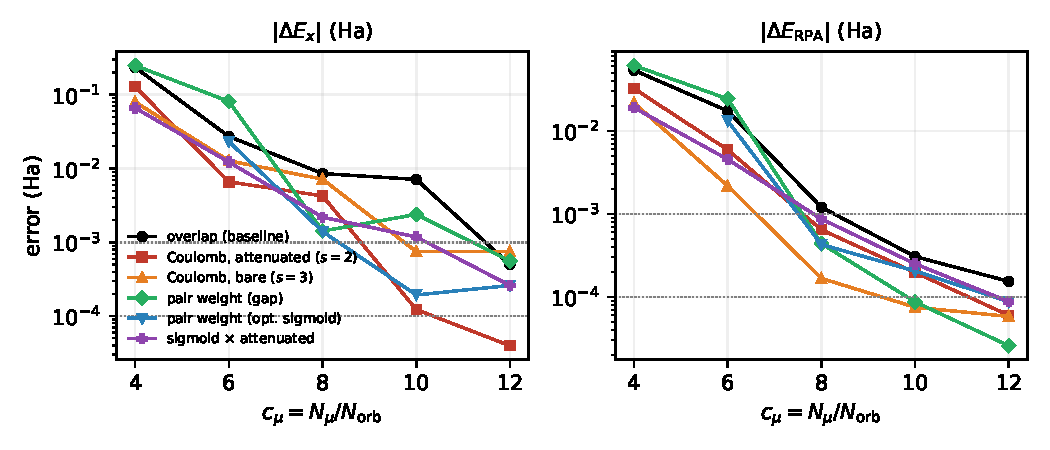
\includegraphics[width=\columnwidth]{figs/si_ncpp_err_vs_cmu.pdf}
  \caption{\todo{Error in $E_x$, $E_H$, $E_{\rm RPA}$ vs $\cmu$ for Si (NCPP),
  baseline vs knobs.}}
  \label{fig:si_ncpp}
\end{figure}

\section{Discussion and conclusions}
\label{sec:conclusions}

\todo{when does the metric matter (vacuum, localized orbitals, metals);
go/no-go criterion from spec Sec. 8; screened-interaction extension;
composition guidance and recommended defaults.}

\begin{acknowledgments}
The Flatiron Institute is a division of the Simons Foundation.
\end{acknowledgments}

%\bibliography{isdf_metric}

\end{document}
